\chapter{Jet Tagging via Particle Clouds}

Representing Jets is a core component of ML on Jet Physics. In  
\href{run:../papers/Jet\ Tagging\ via\ Particle\ Clouds.pdf}{this paper}, 
they are represented by particle clouds, which considers Jet as an 
unordered set of its constituent particles.

\section{Jets}
Jet is a collimated spray of particles. It is one of the most ubiqutous 
objects in proton-proton collision events at the LHC.

\begin{definition}
    aA Jet is defined as a narrow cone of hadrons and other particles 
    produced by the hadronization of a quark or gluon in a particle physics 
    or heavy ion experiment.
    \\\\
    - Wikipedia
\end{definition}

\noindent Jet exhibits different characteristics when initiated by different 
particles. Jets initiated by gluons tend to have broader energy spectrum 
than jets initiated by quarks.

\subsection{Characteristics}
TODO : Find different characteristics due to different initiating particles.

\subsection{Generating Data}
The Large Hadron Collider (LHC) is the place, where all the particle-particle 
collisions occur and live data can be generated. As this data is too huge, 
CERN has developed toolchain known as Root, which is a command-line 
interface and with tools known as Pythia and MadGragh is used to generate the 
data.
\\\\
This data is not the actual data which is observed in the LHC, but 
rather the result of the simulations which are generated locally and is 
based on the phsics incorporated by them in CERN. They are close 
enough to the actual data, hence all algorithms are trained on it.
\\\\
TODO : More information on how to generate data

\section{Jet Tagging}
Jet Tagging is one of the most important topics of interest and study in the 
field of Jet Physics.

\begin{definition}
    jJet tagging is finding the source particle that initiated the Jet.
\end{definition}

\noindent The study of Jet Tagging has been done for a long time. The first and 
initial methods consisted of QCD theory to distinguish between quark and gluon 
Jets.
\\\\
The newer approaches involve Machine Learning where Jets are viewed as images, 
sequences, trees, graphs or set of particles. The tagging isdone using deep 
NNs.

\subsection{QCD Theory}

\begin{definition}
    iIn theoretical physics, quantum chromodynamics (QCD) 
    is the theory of the strong interaction between quarks and gluons, 
    the fundamental particles that make up composite hadrons such as the 
    proton, neutron and pion.
\end{definition}
TODO : More information on QCD theory and how it was used to study Jets

\section{Jet Representation}
The effectiveness and efficiency of ML techniques on jet physics relies 
heavily on how a jet is represented. Some of the mainsteam representations 
and a new representation used by this paper is reviewed and explained here.

\subsection{Image-Based Representation}
One of earliest (and successful) representation of jets is image representation. 
In this method, the energy deposition on each cell is used pixel intensity 
which creates an image of the Jet.
\\\\
The enery deposition of a Jet is measured b a calorimeter. It is done on a 
fine-grained spatial cells, thus giving a matrix value table, which can be 
used as a pixel value, thus constructing an image representation of the jet.
\\\\
This approach is used and studied extensively for various jet tagging tasks.
Examples include W boson tagging, top tagging, and quark-gluon tagging. 
CNNs (and modifications) are used with this representation as they 
provide a natural extension of Computer Vision tasks.
\\\\
They have an extensive advantage over traditional methods motivated by QCD 
theory. The QCD theory motivates multivaraite methods using observables. 
\\\\
There are two major downsides to this reprsentation though, which makes it 
less efficient and thus not universally used. The first is its inability 
to take additional information in a meaningful manner. This is due to 
the fact that the data given by the calorimeter is non additive to the 
data that can be retrieved later.
\\\\
Another downside is the sparseness of the generated image. This is due to the 
fact that jet has particles in the order of $O(10) - O(100)$. This means 
that the image requires around $O(100)$ pixels. But a jet image requires 
$O(1000)$ pixels to contain a jet. Hence, most of the pixels are blank. This 
makes CNNs computatationaly innefective on jet images.

\subsection{Particle-Based Representation}
Another popular way of representing the jet is as a collection of its 
constituent particles. 

\subsection{Particle Cloud}
In the previous section, different representation of Jets were given, which were 
helpful in jet tagging using ML. In this paper, a different and novel way of 
representation of jets is proposed known as particle cloud. It is analogous 
to point cloud reprsentation (3D shapes) which is used in Computer Vision(CV).
\\\\
In this paper, they designed ParticleNet, which is based on Dynamic Graph 
Convolution Neural Network (DGCNN). This operates directly on particle clouds 
for jet tagging.
\\\\
The idea is that the most natural representation of jets is an unordered, 
permutation-invariant set of particles. It is a special ase of Particle 
based representation, thus has all of its benifits (Flexibility, Smaller Size, 
Efficiency, etc).
\\\\
As particle cloud is so similar in structure to cloud representation, all the 
algorithms applicable to it are helpful to make algorithms for particle clouds.

\begin{note}
    aThere are other representations as well which are useful. One of them is 
    represnting jets as graphs, with the vertices as particles. Message Passing 
    NNs (MPNNs) with variations are used on these representations, and depending 
    on how the adjacency matrices are defined, it can have better performance 
    than the RecNNs. There is however a cache that the definition of adjacency 
    matrix might not respect permutation symmetry of the particles.
\end{note}

\section{Machine Learning Algorithm}
This paper talks in detail about ParticleNet, a CNN-like deep NN for Jet Tagging. 
The permutation symmetry makes particle cloud representation one of the most 
natural representation, but the best performace can be acheived only if a 
good algorithm is used.

\subsection{Convolutional Neural Networks}
CNNs are the staple algorithm to use when working with images. Hence, almost 
every algorithm developed for images is based on CNNs. There are two major reasons 
why they are so successful.

\begin{definition}
    Convolution is a mathematical operation $*$, defined as :

    \begin{equation*}
        (f*g)(t) \triangleq \int_{-\infty}^{\infty} f(\tau)g(t - \tau) d\tau
    \end{equation*}

    \noindent This operation is translation independant. This is defined for 
    a continuous function.
\end{definition}

\noindent Convolution operations exploit translational symmetry of images 
by using shared kernels across the complete image. This reduces 
number of parameters and allows them to be learnt more effectively.
\\\\
The second reason is that CNNs use heirarchical approach of learning features. 
This means that CNN layers can be effectively statcked to form a deep network.

\begin{note}
    aA single CNN layer can learn a more global feature than the previous one. 
    This means that when stacking them, the earlier ones can learn local 
    features, whereas the deeper ones can learn more global features. As they 
    follow a hierarchy, this property is known as heirarchical approach.
\end{note}

\subsection{Edge Convolution}
As CNNs are very useful and effective against images, a similar approach for 
learning point cloud data is promoted, but as standard CNNs cannot be applied 
on the point cloud representation, some modifications must be made to the 
algorithm to make it usable.
\\\\
One of the major hurdles is that point cloud representation does not have 
a regular matrix like shape, but is rather irregular distribution. Hence, 
the basis for the convolution (local patch of each point on which the 
kernel operates), is to be defined.
\\\\
Another problem is that the regular convolution operation, in the form of 
$\sum \mathcal{K}_jx_j$ ($\mathcal{K}_j$ : $j^{th}$ kernel, $x_j$ : $j^{th}$ 
feature) is not permutation invariant. Hence, this also needs to be 
modified.
\\\\
Edge Convolution is a modification of the standard convolution operation 
for point clouds. This operation requires the point cloud as a graph, with 
each point represting a vertex and the edges are constructed as connections 
between the k nearest neighbours of the point.

\begin{definition}
    tThe EdgeConv operation is as follows :

    \begin{equation*}
        x_i' \triangleq \fbox{$\phantom{5}$}_{j=1}^k h_\theta(x_i,x_{i_j})
    \end{equation*}

    \noindent In this defintion, the variables and operations are as below :\\
    $\fbox{$\phantom{5}$}$ : Channel-wise symmetric aggregation operation\\
    $h_\theta : \mathcal{R}^F \times \mathcal{R}^F \rightarrow \mathcal{R}^F$\\
    $x_i$ : Feature Vector of point $x_i$
\end{definition}

\noindent In the defintion of EdgeConv given above, the function is 
parametrized by the set of learnable parametes $\theta$. In this paper, a 
specialized form of edge function is used.
\\\\
The $h$ function used is defined as :

\begin{equation*}
    h_\theta(x_i,x_{i_j}) = \overline{h}_\theta(x_i,x_i - x_{i_j})
\end{equation*}

\noindent In this, the function $\overline{h}_\theta$ can be implemented as a 
multilayer perceprtron, whose parameters are shared among all the edges. Also 
in this paper, the aggregation operation used is mean, rather than max which 
was the function used in the original paper. The EdgeConv operation thus is :

\begin{equation*}
    x_i' = \frac{1}{k} \sum_{j=1}^k \overline{h}_\theta(x_i,x_i - x_{i_j})
\end{equation*}

\noindent An EdgeConv block is implemented according to the diagram given below :

\begin{center}
    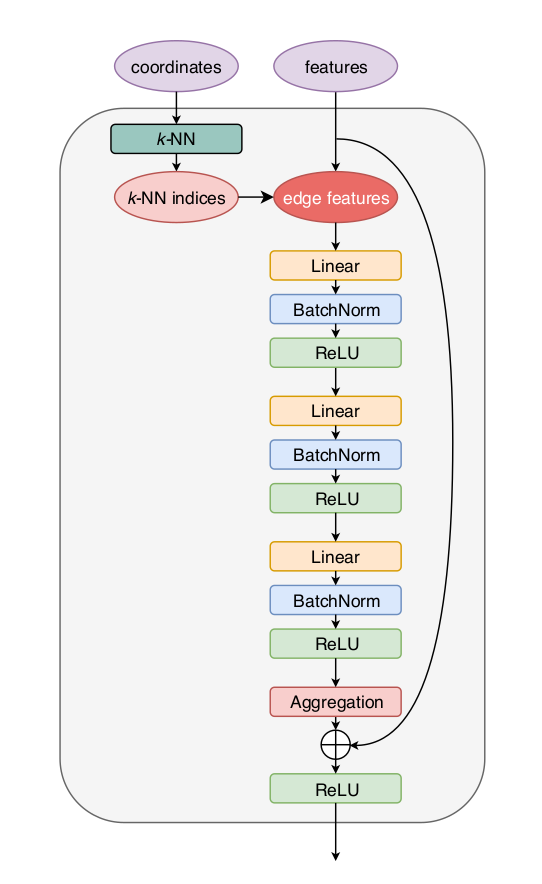
\includegraphics[scale=0.3]{img/theory-ml-particlenet/edge-conv.png}
\end{center}

\noindent The hyperparameters of the EdgeConv operation are the number of 
neighbours $k$, and the number of channels $C = <C_1,C_2,C_3>$, each 
corresponding to  number of units in the linear transformation layer.
\\\\
As this operation preserves the dataset as a point cloud, they 
can be stacked just as easily as standard convolutions.

\begin{note}
    Multilayer Perceptron is a class of feedforward ANNs. The term, though is 
    used ambiguously to classify any feedforward ANN.
\end{note}

\noindent The stackability also allows a us to view the feature vectors 
learnt as new coordinates of the original points in the latent space. This allows 
determination of distance between points in this new space (Computed while 
determining $h_\theta$). This means that proximitiy of points can be dynamically 
learnt using EdgeConv. This results in the DGCNN, in which the graph describing 
the point clouds are dynamically updated to reflect the changes in the edges.

\subsection{ParticleNet}
ParticleNet is a sort of modified and specialized version of DGCNN, which has 
different design choices to suit the jet tagging task. It makes extensive 
use of EdgeConv operation, but has specialized configuration to make it 
suit better.
\\\\
The ParticleNet algorithm is given in the diagram given below :

\begin{center}
    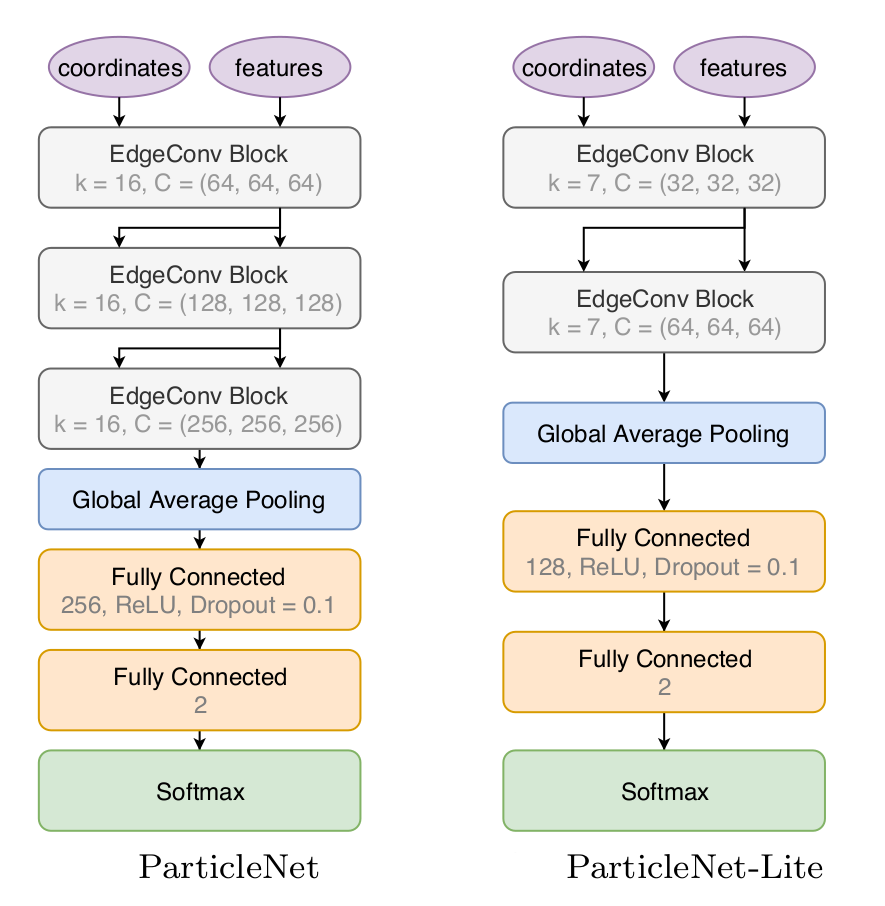
\includegraphics[scale=0.25]{img/theory-ml-particlenet/particle-net.png}
\end{center}

\noindent These are the two implementations of ParticleNet which were used 
in the paper. All the results published in the paper were using this algorithm.